%% ----------------------------------------------------------------
%% Thesis.tex -- MAIN FILE (the one that you compile with LaTeX)
%% ---------------------------------------------------------------- 

% Set up the document
\documentclass[a4paper, 11pt, oneside]{Thesis}  % Use the "Thesis" style, based on the ECS Thesis style by Steve Gunn
\graphicspath{{Figures/}}  % Location of the graphics files (set up for graphics to be in PDF format)

% Include any extra LaTeX packages required
\usepackage[square, numbers, comma, sort&compress]{natbib}  % Use the "Natbib" style for the references in the Bibliography
\usepackage{verbatim}  % Needed for the "comment" environment to make LaTeX comments
\usepackage{vector}  % Allows "\bvec{}" and "\buvec{}" for "blackboard" style bold vectors in maths
\hypersetup{urlcolor=blue, colorlinks=true}  % Colours hyperlinks in blue, but this can be distracting if there are many links.
\usepackage{braket}
\usepackage{afterpage}
\usepackage{tikz}
\usetikzlibrary{shapes,arrows,positioning}
\tikzstyle{decision} = [diamond, draw, fill=green!20,text width=4.5em, text badly centered, node distance=1cm, inner sep=0pt]
\tikzstyle{block} = [rectangle, draw, fill=blue!20,text width=10em, text centered, rounded corners, minimum height=4em]
\tikzstyle{block2} = [rectangle, draw, fill=red!20,text width=10em, text centered, rounded corners, minimum height=4em]
\tikzstyle{line} = [draw, -latex]
\tikzstyle{cloud} = [draw, ellipse,fill=red!20, node distance=3cm,minimum height=2em]
%% ----------------------------------------------------------------
\begin{document}
\frontmatter	  % Begin Roman style (i, ii, iii, iv...) page numbering

% Set up the Title Page
\title  {Improving the Contrast of Neutron Interferometry Phase Measurements Using Online Bayesian Markov Chain Monte Carlo Methods}
\authors  {\texorpdfstring
            {\href{taalexander@mta.ca}{Thomas Alexander}}
            {Thomas Alexander}
            }
\addresses  {\groupname\\\deptname\\\univname}  % Do not change this here, instead these must be set in the "Thesis.cls" file, please look through it instead
\date       {\today}
\subject    {}
\keywords   {}

\maketitle
%% ----------------------------------------------------------------

\setstretch{1.3}  % It is better to have smaller font and larger line spacing than the other way round

% Define the page headers using the FancyHdr package and set up for one-sided printing
\fancyhead{}  % Clears all page headers and footers
\rhead{\thepage}  % Sets the right side header to show the page number
\lhead{}  % Clears the left side page header

\pagestyle{fancy}  % Finally, use the "fancy" page style to implement the FancyHdr headers

%% ----------------------------------------------------------------
% Declaration Page required for the Thesis, your institution may give you a different text to place here
\Declaration{

\addtocontents{toc}{\vspace{1em}}  % Add a gap in the Contents, for aesthetics

I, Thomas Alexander, declare that this thesis titled, "Improving the Contrast of Neutron Interferometry Phase Measurements Using Online Bayesian Markov Chain Monte Carlo Methods" and the work presented in it are my own. I confirm that:

\begin{itemize} 
\item[\tiny{$\blacksquare$}] This work was done wholly or mainly while in candidature for a research degree at this University.
 
\item[\tiny{$\blacksquare$}] Where any part of this thesis has previously been submitted for a degree or any other qualification at this University or any other institution, this has been clearly stated.
 
\item[\tiny{$\blacksquare$}] Where I have consulted the published work of others, this is always clearly attributed.
 
\item[\tiny{$\blacksquare$}] Where I have quoted from the work of others, the source is always given. With the exception of such quotations, this thesis is entirely my own work.
 
\item[\tiny{$\blacksquare$}] I have acknowledged all main sources of help.
 
\item[\tiny{$\blacksquare$}] Where the thesis is based on work done by myself jointly with others, I have made clear exactly what was done by others and what I have contributed myself.
\\
\end{itemize}
 
 
Signed:\\
\rule[1em]{25em}{0.5pt}  % This prints a line for the signature
 
Date:\\
\rule[1em]{25em}{0.5pt}  % This prints a line to write the date
}
\clearpage  % Declaration ended, now start a new page

%% ----------------------------------------------------------------
% The "Funny Quote Page"
\pagestyle{empty}  % No headers or footers for the following pages

\null\vfill
% Now comes the "Funny Quote", written in italics
\textit{``Magic's just science that we don't understand yet.''}

\begin{flushright}
Arthur C. Clarke
\end{flushright}

\vfill\vfill\vfill\vfill\vfill\vfill\null
\clearpage  % Funny Quote page ended, start a new page
%% ----------------------------------------------------------------

% The Abstract Page
\addtotoc{Abstract}  % Add the "Abstract" page entry to the Contents
\abstract{
\addtocontents{toc}{\vspace{1em}}  % Add a gap in the Contents, for aesthetics

The Thesis Abstract is written here (and usually kept to just this page). The page is kept centered vertically so can expand into the blank space above the title too\ldots

}

\clearpage  % Abstract ended, start a new page
%% ----------------------------------------------------------------

\setstretch{1.3}  % Reset the line-spacing to 1.3 for body text (if it has changed)

% The Acknowledgements page, for thanking everyone
\acknowledgements{
\addtocontents{toc}{\vspace{1em}}  % Add a gap in the Contents, for aesthetics

The acknowledgements and the people to thank go here, don't forget to include your project advisor\ldots

}
\clearpage  % End of the Acknowledgements
%% ----------------------------------------------------------------

\pagestyle{fancy}  %The page style headers have been "empty" all this time, now use the "fancy" headers as defined before to bring them back


%% ----------------------------------------------------------------
\lhead{\emph{Contents}}  % Set the left side page header to "Contents"
\tableofcontents  % Write out the Table of Contents

%% ----------------------------------------------------------------
\lhead{\emph{List of Figures}}  % Set the left side page header to "List if Figures"
\listoffigures  % Write out the List of Figures

%% ----------------------------------------------------------------
\lhead{\emph{List of Tables}}  % Set the left side page header to "List of Tables"
\listoftables  % Write out the List of Tables

%% ----------------------------------------------------------------
\setstretch{1.5}  % Set the line spacing to 1.5, this makes the following tables easier to read
\clearpage  % Start a new page
\lhead{\emph{Abbreviations}}  % Set the left side page header to "Abbreviations"
\listofsymbols{ll}  % Include a list of Abbreviations (a table of two columns)
{
% \textbf{Acronym} & \textbf{W}hat (it) \textbf{S}tands \textbf{F}or \\
$t$ & transmitted beam amplitude coefficient \\
$r$ & reflected beam amplitude coefficient \\

}

%% ----------------------------------------------------------------
\clearpage  % Start a new page
\lhead{\emph{Physical Constants}}  % Set the left side page header to "Physical Constants"
\listofconstants{lrcl}  % Include a list of Physical Constants (a four column table)
{
% Constant Name & Symbol & = & Constant Value (with units) \\
Speed of Light & $c$ & $=$ & $2.997\ 924\ 58\times10^{8}\ \frac{m}{s}$ \\

}

%% ----------------------------------------------------------------
\clearpage  %Start a new page
\lhead{\emph{Symbols}}  % Set the left side page header to "Symbols"
\listofnomenclature{lll}  % Include a list of Symbols (a three column table)
{
% symbol & name & unit \\
$k$ & quantum wave number & $m^{-1}$ \\
$v$ & velocity & $ms^{-1}$ \\
& & \\ % Gap to separate the Roman symbols from the Greek
$\omega$ & angular frequency & rads$^{-1}$ \\
}
%% ----------------------------------------------------------------
% End of the pre-able, contents and lists of things
% Begin the Dedication page

\setstretch{1.3}  % Return the line spacing back to 1.3

\pagestyle{empty}  % Page style needs to be empty for this page
\dedicatory{For/Dedicated to/To my\ldots}

\addtocontents{toc}{\vspace{2em}}  % Add a gap in the Contents, for aesthetics


%% ----------------------------------------------------------------
\mainmatter	  % Begin normal, numeric (1,2,3...) page numbering
\pagestyle{fancy}  % Return the page headers back to the "fancy" style

% Include the chapters of the thesis, as separate files
% Just uncomment the lines as you write the chapters

% Chapter 1

\chapter{Introduction} % Write in your own chapter title
\label{Chapter1}
\lhead{Chapter 1. \emph{Introduction}} % Write in your own chapter title to set the page header


\section{Neutron Interferometry}
\subsection{History}
Interferometry has long been a powerful tool for experimental physics. Its various forms have been used in the discovery of many historically significant results such as the Michelson-Morley experiment which showed that the speed of light was independent of inertial reference frames and experimental data in support of Bell's Inequality. \cite{michelson_morley}\cite{bells_inequality}

The key concept of interferometry is the superposition of waveforms upon each other in order to deduce meaningful physical properties from the resultant combination. If one considers two waves of identical frequency than the waves when superimposed will combine constructively when in phase and de-constructively when out of phase. The technique of interferometry can be applied to many different experimental systems, the requirement being that the interferometry medium be described as a wave mathematically. Such systems that have been used in the past include electromagnetic waves, water waves, electrons and neutrons. Although electrons and neutrons classically are described as point particles the development of quantum mechanics allows that all matter is actually described by a waveform and therefore interferometry techniques may be applied to the electron and neutron waveforms. This paper focuses primarily on neutron interferometry. 

The first Neutron Interferometer with slow neutrons was constructed by Maier-Leibnitz and Springer in 1962 and was effectively equivalent to a double slit experiment. However, their interferometer was not effective for measuring physical properties of materials. In 1965 the perfect single-crystal interferometer was theorized by Ulrich Bonse and Michael Hart, however it was not until 1974 that their interferometer was made functional by Helmut Raunch and his student Wolfgang Treimer. Their interferometer used a single perfect crystal in which two horizontal slices were removed from the interior to form a three-blade interferometer.\cite{neutron_history} Using the single-crystal design researchers Colella,Overhauser and Werner to perform the famous COW experiment which measured the phase shift due to the gravitational potential difference between two neutron beams separated by a small displacement in height.\cite{cow} Further experiments made such contributions to experimental physics such as the measurement of the Aharonov-Bohm effect and the the effect of the Earth's rotation on a quantum system.\cite{neutron_history} It was quickly realized that neutron interferometry measurements provide an incredible level of accuracy and isolation in experimental measurements. This is due to the fact that the neutron has essentially zero electric charge and therefore does not feel the Coulomb force. Therefore for the case of slow neutrons there is no need to isolate for stray electric fields. 
\begin{figure}[ht!]
\centering
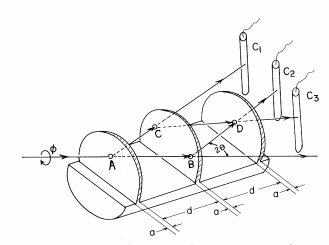
\includegraphics[scale=1.0]{Figures/cow.png}
\caption{An illustration of the interferometer used in the COW experiment.\cite{cow}}
\label{fig:cow}
\end{figure}

\subsection{Application to Quantum Information}
As the neutron interferometry provides a low-noise experimental system it provides an ideal test-bench for testing certain aspects of quantum information theory. Such an example was the use of a five-blade interferometer which allowed the quantum information encoded in the neutron waveform by using additional blades to exploit the symmetry of mechanical vibrations in the interferometer and decouple these modes.\cite{five_blade}. This is an example of encoding the information into a decoherence-free subspace and is a technique that may be applicable in future scalable quantum computation systems. Additionally it has been shown that neutron interferometers can be used for the generation of single neutron entangled states. \cite{neutron_entanglement}   Additionally there is interest in the quantum discord of neutron interferometry systems and there application towards non-classical discord algorithms.\cite{noise_neutron}. It is unlikely that a scalable quantum computer will be realizable with neutrons due to their low interaction with other quantum systems.  
\subsection{Application to Quantum Fundamentals}
Neutron interferometry has played a large role in experimentally gathering information on the fundamental behaviour of quantum systems. Such as the Aharonov-Bohm effect, the effect of gravity,quantum discord and verifying Bell's Inequality. \cite{neutron_history}\cite{cow}\cite{noise_neutron}\cite{bells_inequality}. More recently researchers at the Institute for Quantum Computing are designing an experimental neutron interferometer that is equivalent to a triple-slit experiment in the search for third order interference effects that are theoretically non-existent but if found may be evidence of new quantum theories.\cite{three_slit} 
\subsection{National Institute of Standards and Technology}
The majority of the work presented in this thesis applies directly to the neutron interferometry setup at the National Institute of Standards and Technology in Gaithersburg, MD. The neutrons are produced at the NIST Research Reactor and extracted via a dual-crystal parallel-tracking monochromator with energy of $4-20 meV$. They are fed along wave-guides to the isolated interferometry setup. NIST has three,four and five blade perfect single-crystal interferometry assemblies although we focus on solely the three blade assembly. Neutron detection is provided by $^3He$ detectors or by high resolution position-sensitive detectors.\cite{nist_setup}\cite{nist_powerpoint} 

\begin{figure}[ht!]
\centering
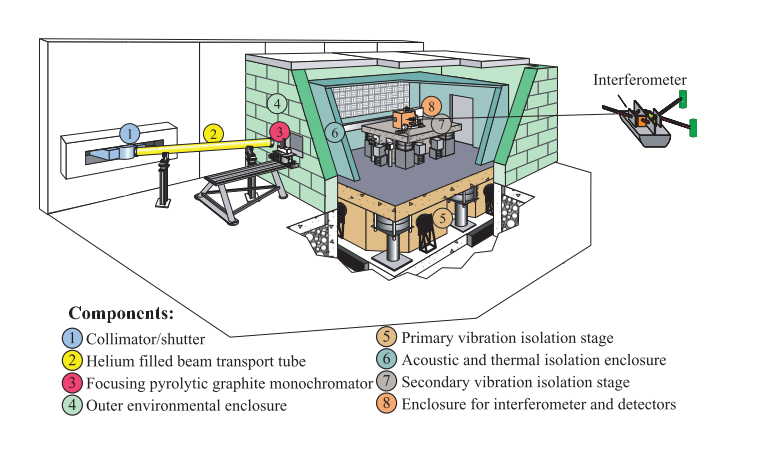
\includegraphics[scale=1.0]{Figures/neutroninterferometer.png}
\caption{Neutron interferometry lab at NIST \cite{dimaThesis}}
\label{fig:neutroninterferometerlab}
\end{figure}
\section{Markov Chain Monte Carlo Methods}
Often in advanced quantum physics the probability distributions of the systems reside in a high dimensional parameter space. It is often desired to find the correct set of parameters to describe a system. However, it is normally impossible to test every single possible real value of the parameter space as the computational time would be astronomical. Markov Chain Monte Carlo methods attempt to solve this problem by using a bunch of "guesses" that will according to a heuristic attempt to reasonably explore the parameter space for the approximate parameters after many iterations.  Markov Chain Monte Carlo Methods have many uses including in Bayesian statistics, physics, biology and linguistics.\cite{mcmc}

The Markov Chain Monte Carlo method can be thought of scattering a large number of particles in a space to be explored. By moving these particles around the space, it is possible to effectively sample the entire space if enough iterations and particles are used. We will use MCMC methods to explore the parameter space of neutron detection probability distributions in order to obtain the optimal set of system parameters. 
\begin{figure}[ht!]
\centering
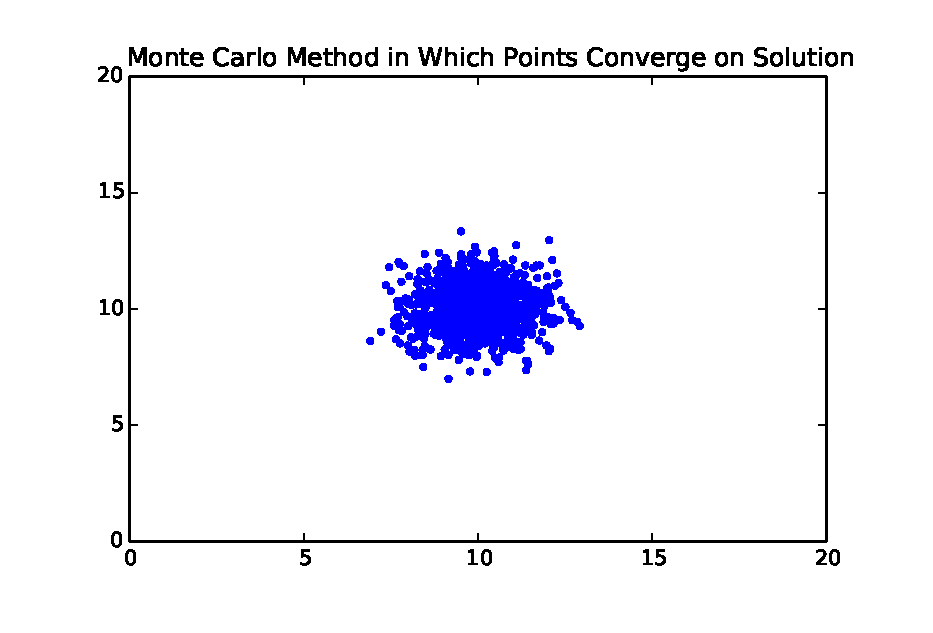
\includegraphics[scale=1.0]{Figures/mcmc.eps}
\caption{Markov Chain Monte Carlo method converging on solution at $(10,10)$}
\label{fig:mcmc}
\end{figure} % Introduction

% Chapter 2

\chapter{Theory} % Write in your own chapter title
\label{Chapter2}
\lhead{Chapter 2. \emph{Theory}} % Write in your own chapter title to set the page header


\section{Neutrons}
\subsection{Particle Description of Neutrons}
The neutron is a subatomic hadron particle that is present in the nucleus of every atom except $^1H$. The neutron is composed of two down quarks and a single up quarks. This composition gives a neutral electric charge for the neutron making it an ideal candidate for sensitive experiments, however the downside is that neutrons are much more difficult to manipulate. The neutron is also a fermion and by the Pauli exclusion principle only a single neutron is allowed in each quantum state. The free neutron is unstable and undergoes beta decay with a lifetime of just $881.5 \pm 1.5 s$. The neutron has a rest mass of approximately $939.56Mev$. Free neutrons are produced using either neutral fission or fusion although in practical experiments fission is almost always used. At the NIST Research Reactor free neutrons are produced from the fission of $^{235}U$.\cite{dimaThesis}
\subsection{Thermal Neutrons}
\label{sec:thermal}
Neutron interferometry utilizes thermal neutrons which are free neutrons that follow a Boltzmann distribution. The neutrons at NIST are found in the kinetic energy range of $4$-$20meV$ around room temperature of $T=293.15K$. This gives neutron velocities of $875-1956\frac{m}{s}$ which gives $v<<c$ and therefore relativistic affects do not play a role. Therefore thermal neutrons are in near thermal equilibrium with their surroundings. Neutrons are decelerated to a thermal state in the reactor by collisions with neutron moderators in the reactor. From de Broglie relations the wavelength of thermal neutrons is approximately $\lambda = \frac{h}{p}= 2.0$-$4.5\AA$. After being emitted form the NIST reactor the neutrons follow a wave-guide and using a wave splitter are sent into individual labs. As the strongest known phase space density of a neutron source is around $10^{-14}$ it can be safely assumed that the probability of two neutrons interacting inside the wave-guide or interferometer is sufficiently low that it can be disregarded and therefore detected neutrons have no correlation between each-other.\cite{dimaThesis}

\section{Neutron Interferometry}
The Neutron interferometer is similar to other forms of interferometry in which an incoming wave is split and than allowed to interfere at a later point which allows the two wave paths to be compared. The modern day neutron interferometer is functionally equivalent to an optical Mach-Zender (MZ) interferometer.\cite{machzehnder}

\subsection{Bragg Scattering}
In neutron interferometry the crystal planes of the interferometer blades act as diffraction gratings. Incident waves that satisfy the Bragg condition \ref{bragg} are coherently scattered.
\begin{equation}
\label{bragg}
n\lambda = 2d sin(\theta_{B})
\end{equation} 
Where $n$ is a positive integer, $d$ is the distance between the atomic planes of the crystal lattice and $\theta_{B}$ is the angle between the incident beam and the atomic plane of the crystal. Not all of the amplitude of the neutron beam is scattered and a large portion is transmitted through the crystal with only its phase shifted. The amplitudes of the transmitted and the reflected beams are given by the coefficients $t$ (transmitted) and $r$ reflected. Under the assumption that the entire beam is either Bragg scattered or transmitted the coefficients $t$ and $r$ must have the following relationship.\cite{dimaThesis}  
\begin{equation}
|r|^2+|t|^2 = 1
\label{eq:BraggCoefficents}
\end{equation}

\begin{figure}[ht!]
\centering
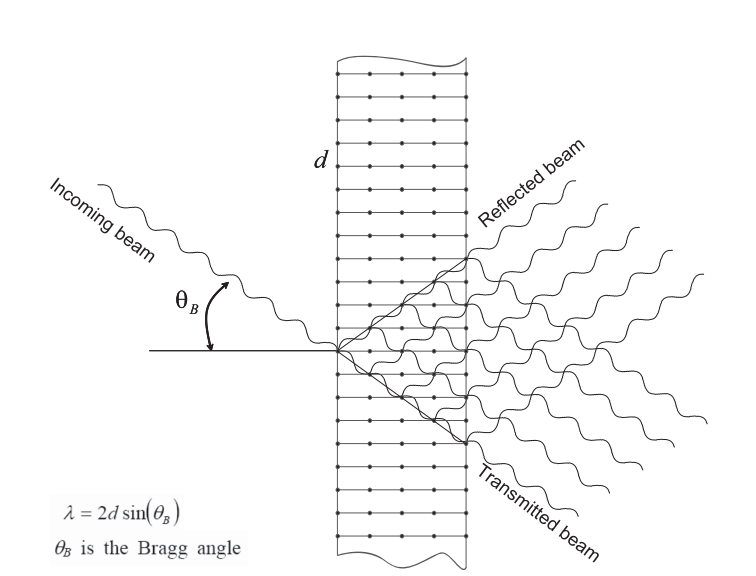
\includegraphics[scale=0.5]{Figures/braggscattering.png}
\caption{Bragg scattering off of a crystal lattice}
\label{fig:braggscattering}
\end{figure}

\subsection{Quantum Scattering Theory}
\label{sec:scatteringTheory}
 Starting with the assumption the Hamiltonian has the form of 
 \begin{equation}
 \mathcal{H} = \mathcal{H}_0+\mathcal{V} \,\,\,\,\, \mathcal{H}_0= \frac{\textbf{p}^2}{2m}
 \label{eq:hamiltonian}
 \end{equation}
The presence of the potential $\mathcal{V}$ causes the solution to be different than the free particle state 
$$\mathcal{H}_0\Ket{\Phi}=E\Ket{\Phi}$$

Therefore we are looking for solutions to the Schrödinger equation of the form \cite{sakurai}
\begin{equation}
\label{eq:schrodinger}
(\mathcal{H}_0+\mathcal{V})\Ket{\Psi} = E\Ket{\Psi} 
\end{equation} 
 A valid solution should have that $\Ket{\Psi}\rightarrow\Ket{\Phi}$ as $\mathcal{V}\rightarrow 0$. A solution that satisfies these requirements is known as the Lippmann-Schwinger equation. \cite{sakurai}
 \begin{equation}
 	\label{lippmanSchwinger}
 	\Ket{\Psi^{\pm}}=\Ket{\Phi}+\frac{1}{E-\mathcal{H}_0\pm i\epsilon}\mathcal{V}\Ket{\Psi^{\pm}} 
 \end{equation}
 Here the energy $E$ was made slightly complex with the addition of $\pm \epsilon$ to deal with the singular nature of the operator $1/(E-\mathcal{H}_0)$. It can easily be seen that the application of the operator $E-\mathcal{H}_0$ reduces (\ref{lippmanSchwinger}) to the desired solution (\ref{eq:schrodinger}) when neglecting the imaginary component. By taking the Lipmann-Schwinger equation to the position basis explicitly it can be represented as \cite{sakurai}
 \begin{equation}
 \label{eq:positionBasis}
 \Braket{\mbox{\boldmath$x$}|\Psi^{\pm}}=\Braket{\mbox{\boldmath$x$}|\Phi} -\frac{2m}{\hbar^2} \int d^3x^{'} \frac{e^{\pm ik\left|\mbox{\boldmath$x-x^{'}$}\right|}}{ 4\pi \left| \mbox{\boldmath$x-x^{'}$} \right|} \Braket{\mbox{\boldmath$x^{'}$}|\mathcal{V}|\Psi^{\pm}}
 \end{equation}
As our scattering potentials are a function of position only the assumption can be made that the potential is \textit{local} such that it is diagonal in the position representation. Specifically the potential satisfies the requirement that \cite{sakurai}
\begin{equation}
\label{eq:localPotential}
\braket{\mbox{\boldmath$x^{'}$}|\mathcal{V}|\mbox{\boldmath$x^{''}$}}=\mathcal{V}(\mbox{\boldmath$x$}^{'})\delta^{(3)}(\mbox{\boldmath$x^{'}$}-\mbox{\boldmath$x^{''}$})
\end{equation}

Utilizing this potential we obtain 
\begin{equation}
\label{eq:localPotentialResult}
\Braket{\mbox{\boldmath$x$}|\mathcal{V}|\Psi^{\pm}}=\int d^3x^{''} \braket{\mbox{\boldmath$x^{'}$}|\mathcal{V}|\mbox{\boldmath$x^{''}$}} \braket{\mbox{\boldmath$x^{''}$}|\Psi^{\pm}}=\mathcal{V}(\mbox{\boldmath$x^{'}$})\braket{\mbox{\boldmath$x^{'}$}|\Psi^{\pm}}
\end{equation}
With this result the Lippmann-Schwinger equation can be reduced to 
\begin{equation}
\label{eq:lippmannSchwingerLocal}
 \Braket{\mbox{\boldmath$x$}|\Psi^{\pm}}=\Braket{\mbox{\boldmath$x$}|\Phi} -\frac{2m}{\hbar^2} \int d^3x^{'} \frac{e^{\pm ik\left|\mbox{\boldmath$x-x^{'}$}\right|}}{ 4\pi \left| \mbox{\boldmath$x-x^{'}$} \right|} \mathcal{V}(\mbox{\boldmath$x{'}$})\Braket{\mbox{\boldmath$x^{'}$}|\Psi^{\pm}}
\end{equation}
Given that we are concerned with studying finite range scatters and that any observations that will be made outside the range of the potential due to the macroscopic nature of neutron detectors the assumption can be made that $\left|\mbox{\boldmath$x$}\right| >>\left|\mbox{\boldmath$x^{'}$}\right|$. The finite range potential can be seen in fig(\ref{fig:finiteRangePotential}).
\begin{figure}[ht!]
\centering
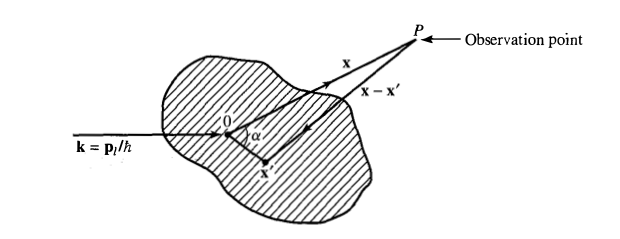
\includegraphics[scale=0.5]{Figures/scatteringObservation.png}
\caption{The finite range scattering potential. Any observations via detectors will be outside the range of the potential and therefore approximations can be made when evaluating (\ref{eq:lippmannSchwingerLocal}).}
\label{fig:finiteRangePotential}
\end{figure}

Keeping in mind this result we can define \cite{sakurai}
$$ r = \left| \mbox{\boldmath$x$} \right| $$
$$r^{'}=\left|\mbox{\boldmath$x^{'}$}\right|$$
$$\alpha = \angle(\mbox{\boldmath$x,x^{'}$})$$
$$\mbox{\boldmath$\hat{r}$} \equiv \frac{\mbox{\boldmath$x$}}{\left|\mbox{\boldmath$x$}\right|}$$

\begin{equation}
\label{eq:toObservation}
\left|\mbox{\boldmath$x-x^{'}$}\right| \approx r-\mbox{\boldmath$\hat{r}\cdot x^{'}$}
\end{equation}
\begin{equation}
\label{eq:propogationVector}
\mbox{\boldmath$k^{'}$} \equiv k\mbox{\boldmath$\hat{r}$}
\end{equation}

Utilizing equations (\ref{eq:toObservation},\ref{eq:propogationVector})
\begin{equation}
e^{\pm ik \left|\mbox{\boldmath$x-x^{'}$}\right|} \approx e^{\pm ikr}e^{\mp i \mbox{\boldmath$k^{'}\cdot x^{'}$}}
\label{eq:waveSimplification}
\end{equation}
For the distant $r$ at the observation point it is a useful approximation to say that 
\begin{equation}
\frac{1}{\left|\mbox{\boldmath$x-x^{'}$}\right|} \approx \frac{1}{r}
\end{equation}
Now replacing our incident generic wave with an incident plane wave $\Ket{\Phi}\rightarrow \Ket{\mbox{\boldmath$p$}}$ and using \mbox{\boldmath$k$} $\equiv \mbox{\boldmath$p_i$}/ \hbar$ to remove the $\hbar$'s from the expression.\cite{sakurai} We obtain for the first term in (\ref{eq:lippmannSchwingerLocal}) 
\begin{equation}
\Braket{\mbox{\boldmath$x$}|\mbox{\boldmath$k$}}=\int d^3k^{'} \Braket{\mbox{\boldmath$x$}|\mbox{\boldmath$k^{'}$}}\Braket{\mbox{\boldmath$k^{'}$}|\mbox{\boldmath$k$}}=\int d^3k^{'}  \Braket{\mbox{\boldmath$x$}|\mbox{\boldmath$k^{'}$}} \delta^{(3)}(\mbox{\boldmath$k^{'}-k$})=\frac{e^{i\mbox{\boldmath$k \cdot x$}}}{(2\pi)^{\frac{3}{2}}}
\label{eq:PlaneWave}
\end{equation}
Using this result in (\ref{eq:lippmannSchwingerLocal}) gives an expression for the scattered wave function at a relatively distant observation point for the positive Lippmann-Schwinger wavefunction. 
\begin{equation}
\label{eq:scatteredEquation}
\Braket{\mbox{\boldmath$x$}|\Psi^{+}} = \frac{1}{(2\pi)^{\frac{3}{2}}}\left(e^{i\mbox{\boldmath$k \cdot x$}} + \frac{e^{ikr}}{r}f(\mbox{\boldmath$k^{'},k$})\right)
\end{equation}
\begin{equation}
\label{eq:f}
f(\mbox{\boldmath$k^{'},k$})=-m\left(\frac{2\pi}{h}\right)^2\Braket{\mbox{\boldmath$k^{'}$}|\mathcal{V}|\Psi^{+}}
\end{equation}
It is very easy to see that the result wavefunction is a combination of the original incident plane-wave and an outgoing spherical wave with an amplitude described by (\ref{eq:f}). An obvious issue is that here scattering has only been treated for an incident plane-wave which is not a normalizable wavefunction. In reality to describe discrete particles such as neutrons wave packet solutions are used to describe the incident particles. However, provided the size of the wave packet is much larger than the range of the finite potential $\mathcal{V}$ it is sufficient to treat an incident packet as a plane-wave.  
\subsection{Differential Scattering Cross-Section}
The scattering cross section is an important parameter for experimental scattering physics. It relates the number of particles scattering into the solid angle $d\Omega$ per unit time to the number of incident particles into an infinitesimal element $d\sigma$ of area per unit time. We search for a relation between $d\Omega$ and $d\sigma$ which we term the differential cross section given by $d\sigma/d\Omega$.\cite{sakurai}
\begin{figure}[ht!]
\centering
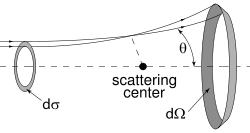
\includegraphics[scale=1.0]{Figures/scatteringCrossSection.png}
\caption{The differential cross section is the relationship between incident particles travelling through area $d\sigma$ to scattered particles crossing through the solid angle $d\Omega$. \cite{sakurai}}
\label{fig:scatteringCrossSection}
\end{figure}
Evidently the probability of an incident particle being within an area $d\sigma$ in time $dt$ while travelling with velocity $v$ is just \cite{griffiths}
\begin{equation}
dP = \left|\Psi_i\right|^2 dV  = \left(\frac{1}{2\pi}\right)^3 (vdt)d\sigma
\label{eq:incidentCross}
\end{equation}

\begin{figure}[ht!]
\centering
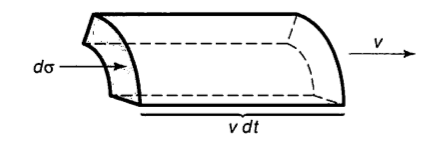
\includegraphics[scale=0.7]{Figures/incidentBeam.png}
\caption{The volume element $dV$ that a beam occupies passing through an area $d\sigma$ in time $dt$. \cite{griffiths}}
\label{fig:incidentBeam}
\end{figure}

Relating this probability to the probability of a particle being scattered into solid angle $d\Omega$ with equal velocity $v$ per unit time $dt$. 
\begin{equation}
\label{eq:scatteredCross}
dP=\left|\Psi_s\right|^2dV = \left(\frac{1}{2\pi}\right)^3 \frac{\left|f(\mbox{\boldmath$k^{'},k$})\right|^2}{r^2}(vdt)r^2 d\Omega
\end{equation}
Equations (\ref{eq:incidentCross}) and (\ref{eq:scatteredCross}) can be solved for the differential cross section 
\begin{equation}
\label{eq:differentialCrossSection}
\frac{d\sigma}{d\Omega}= \left|f(\mbox{\boldmath$k^{'},k$})\right|^2
\end{equation}

\subsection{Scattering Amplitude}
While equation (\ref{eq:f}) defines the magnitude of the outgoing spherical wave, it is defined implicitly in terms of the unknown ket $\Ket{\Psi^{+}}$. The solution to this problem in the case of sufficiently weak scatterers is to use the first Born approximation \cite{sakurai}
\begin{equation}
\label{eq:born}
\Braket{\mbox{\boldmath$x^{'}$}|\Psi^{+}} \rightarrow \Braket{\mbox{\boldmath$x^{'}$}| \Phi} = \frac{e^{i\mbox{\boldmath$k\cdot x^{'}$}}}{(2\pi)^{3/2}}
\end{equation}
Combining (\ref{eq:born}) and (\ref{eq:f}) results in the first-order Born amplitude \cite{sakurai}
\begin{equation}
\label{eq:firstOrderBorn}
f^{(1)}(\mbox{\boldmath$k^{'},k$}) = -\frac{m}{2\pi\hbar^2}\int d^3x^{'}e^{i(\mbox{\boldmath$k-k^{'}$})\cdot \mbox{\boldmath$x^{'}$}}\mathcal{V}(\mbox{\boldmath$x^{'}$})
\end{equation}
As the potentials that will be dealt with are spherically symmetrical, further approximations can be made utilizing $\mbox{\boldmath$q$} \equiv \mbox{\boldmath$k-k^{'}$}$ and $$\left|\mbox{\boldmath$k-k^{'}$}\right| \equiv  q = 2ksin \left( \frac{\theta}{2}\right)$$ as seen in fig(\ref{fig:scatteringAngle}) The spherical symmetry can be used to integrate explicitly the angular component of the scattering magnitude. \cite{sakurai}
\begin{figure}[ht!]
\centering
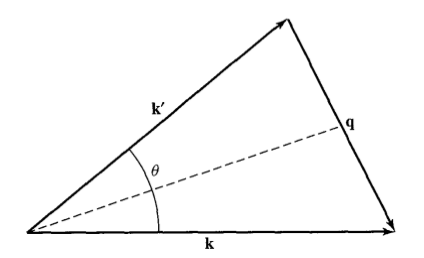
\includegraphics[scale=0.5]{Figures/scatteringAngle.png}
\caption{Scattering amplitude as a function of $\theta$ where $\mbox{\boldmath$q$}=\mbox{\boldmath$k-k^{'}$}$ \cite{sakurai}}
\label{fig:scatteringAngle}
\end{figure}
$$
f^{(1)}(\theta) =  -\frac{m}{2\pi\hbar^2} \int_{r=0}^{\infty} \int_{\phi=0}^{2\pi} \int_{\theta^{'}=0}^{\pi} e^{i \left| q \right| \left| r \right|cos(\theta^{'})}sin(\theta^{'})r^2 \mathcal{V}(r) d\theta^{'} d\phi dr
$$
\begin{equation}
\label{eq:bornAngular}
= -\frac{1}{2i}\frac{2m}{\hbar^2q} \int_{0}^{\infty} r\mathcal{V}(r)(e^{iqr}-e^{-iqr})dr = -\frac{2m}{\hbar^2}\frac{1}{q}\int_{0}^{\infty} r\mathcal{V}(r)sin(qr)dr
\end{equation}
Given a potential that has spherical symmetry it is now much more simple to calculate the scattering amplitude using (\ref{eq:bornAngular}).
\subsection{Neutron-nucleus Scattering}
Generally there are two interactions that an incident neutron on a material will experience. The interaction with the nucleus of the material atoms and which is referred to as nuclear scattering and the scattering due to interaction with unpaired electrons and their magnetic moments which is known as magnetic scattering. In practice nuclear scattering is more common as it allows probing the structure of solids. 

Given the assumptions that an incoming neutron beam will be elastically scattered and that the nucleus is fixed, the scattering will depend on the potential $V(\mbox{\boldmath$r$})$ between the nucleus and neutron. As this interaction is due to the strong-force it is naturally occurring over a very short range, and is approximately zero at a distance of the order $\mbox{\boldmath$r$}=10^{-15}m$. As this is much shorter than the wavelength of thermal and cold neutrons which are used in almost all scattering experiments, the nucleus acts as a point scatterer. A neutron beam can be represented as a plane wave a wave function described by (\ref{eq:PlaneWave}) and the scattered wavefunction will take the form of (\ref{eq:scatteredEquation},\ref{eq:f}).

Due to the magnitude of the difference between the wavelength of the incident neutrons and the effective acting distance of the strong-force neutron-nucleus interaction and its approximate spherical symmetry it is an acceptable approximation to use the Fermi pseudo-potential \cite{waveguide}
\begin{equation}
\label{eq:FermiPseudoPotential}
\mathcal{V}(\mbox{\boldmath$x^{'}$}) = \frac{2\pi\hbar^2}{m}b\delta(\mbox{\boldmath$x^{'}$})
\end{equation}
 as a scattering potential. Where $b$ is known as the neutron scattering length and has units of meters. For the case of multiple nuclei the potential takes the form
 \begin{equation}
 \label{eq:MultipleNuclei}
 \mathcal{V}(\mbox{\boldmath$x^{'}$})  = \frac{2\pi\hbar^2}{m}\sum\limits_{j} b_j \delta(\mbox{\boldmath$x^{'}-x_j$})
 \end{equation}

Using the spherical approximate Born solution for the amplitude (\ref{eq:firstOrderBorn}) and the Fermi pseudo-potential the scattering amplitude can be found to be 
\begin{equation}
f^{(1)}(\theta) = -\int d^3x^{'}e^{i(\mbox{\boldmath$k-k^{'}$})\cdot \mbox{\boldmath$x^{'}$}}\sum\limits_{j} b_j \delta(\mbox{\boldmath$x^{'}-x_j$})=-\sum\limits_{j}b_j e^{i(\mbox{\boldmath$q \cdot x_j$})}
\label{eq:neutronScatteringAmplitude}
\end{equation}
And in the case of a single scatterer at the origin reducing to 
\begin{equation}
f^{(1)}(\theta)  = -b
\label{eq:neutronScatteringSingle}
\end{equation}
Therefore it can be seen that the completed neutron scattered wave form is
\begin{equation}
\label{eq:scatterNeutronWaveForm}
\Braket{\mbox{\boldmath$x$}|\Psi^{+}} = \frac{1}{(2\pi)^{\frac{3}{2}}}\left(e^{i\mbox{\boldmath$k \cdot x$}} - \sum\limits_{j}b_j e^{i(\mbox{\boldmath$q \cdot x_j$})}\frac{e^{ikr}}{r}\right)
\end{equation}

From this approximate solution it is evident that the only difference between individual scatterers is their neutron scattering length $b$. The value $b$ varies greatly among even neighbouring elements in the periodic table. Unfortunately the outlined theory is not strong enough to predict the scattering length and the parameters must be determined experimentally. Fig(\ref{fig:scatteringLength}) shows the scattering length for various elements of the periodic table.

\begin{figure}[ht!]
\centering
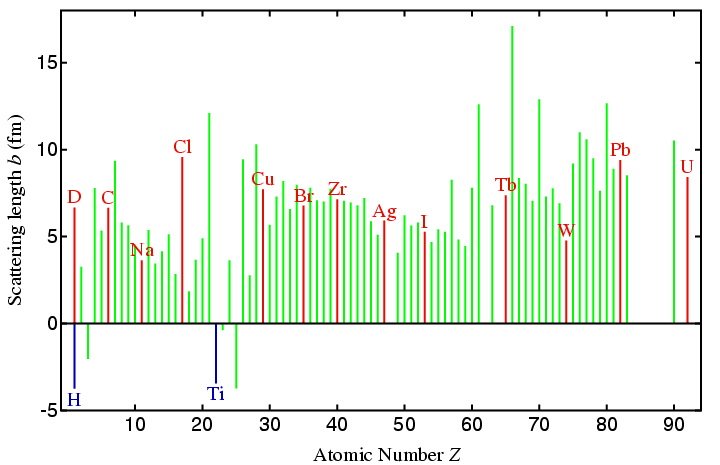
\includegraphics[scale=0.5]{Figures/neutronScatteringLength.png}
\caption{Neutron scattering lengths $b$ for the elements of the periodic table. \cite{scatteringlengths}}
\label{fig:scatteringLength}
\end{figure}

Inside a sufficiently large homogeneous material the Fermi pseudo-potential can be approximated to be 

\begin{equation}
 \mathcal{V}(\mbox{\boldmath$x^{'}$})  = \frac{2\pi\hbar^2}{m}\sum\limits_{j} b_j \delta(\mbox{\boldmath$x^{'}-x_{j}$}) \approx \frac{2\pi\hbar^2}{m}bN 
\label{eq:approxFermiPseudopotential}
\end{equation}

Where $N$ is the atom number density. 
\subsection{Neutron Optics}
As the neutron beam is a wavefunction many analogies from classical optics hold. The index of refraction is defined as the ratio of the speed of neutrons experiencing no potential to the speed of neutrons affected by a potential. Compared to light the form is familiar 
$$ n = \frac{c}{v} = \frac{K}{k}$$
Where from Schrödinger's equation
$$\nabla^2\Psi(\mbox{\boldmath$x$}) + \frac{2m}{\hbar^2}(E-\mathcal{V}(\mbox{\boldmath$x$}))\Psi(\mathbf{x}) = 0 $$ 
\begin{equation}
\label{eq:K}
K^2 = \frac{2m}{\hbar^2}(E-\mathcal{V}(\mbox{\boldmath$x$}))
\end{equation}
\begin{equation}
\label{eq:NinPotential}
n(\mbox{\boldmath$x$}) = \frac{K}{k} = \sqrt{\frac{E-\mathcal{V}(\mbox{\boldmath$x$})}{E}}=\sqrt{1-\frac{\mathcal{V}(\mbox{\boldmath$x$})}{E}}
\end{equation}
Given that the neutron scattering potentials are described by (\ref{eq:approxFermiPseudopotential}) the index of refraction can be approximated to \cite{waveguide}
\begin{equation}
n(\mbox{\boldmath$x$}) = \sqrt{1-\frac{\frac{2\pi\hbar^2}{m}bN}{E}}= \sqrt{1 - \frac{4\pi bN}{k^2}}
\label{eq:indexofrefraction}
\end{equation}

In the case of magnetic materials the magnetic potential
\begin{equation*}
\mathcal{V}_{mag}(\mbox{\boldmath$x$})=-\mbox{\boldmath$u \cdot B_{eff}$}
\end{equation*}
 must be accounted for. This results in an index of refraction for magnetic materials such as Fe,Ni and Co of 
\begin{equation}
n_{\pm}(\mbox{\boldmath$x$})= \sqrt{1-\frac{\frac{2\pi\hbar^2}{m}bN \mp \mbox{\boldmath$u \cdot B_{eff}$}}{E}}
\label{eq:nucleurIndexofRefraction}
\end{equation}
\subsection{Neutron in Material Phase-Shift}
The phase shift due to a perturbing potential is given by \cite{green_2}
\begin{equation}
\phi = \frac{1}{\hbar}\int  \mathbf{p}\cdot \mathbf{dl} = \int \mathbf{K}\cdot d\mathbf{l}= \int \mathbf{nk}\cdot \mathbf{dl}
\label{eq:phase_shift}
\end{equation}
Where $\mathbf{n}$ is the neutron index of refraction and $\mathbf{k}$ is the neutron wave vector. Under the assumption that $\mathbf{n}$ is isotropic and that the perturbation that creates $\mathbf{n}$ does not shift the path to a large degree, the phase difference between two optical paths may be written as
\begin{equation}
\delta\phi = \int (n_1-n_2)\mathbf{k}\cdot \mathbf{dl} = Nb\lambda D
\label{eq:phase_shift_full}
\end{equation}
Where $D$ is the thickness of the material the neutron beam travels through.  

\subsection{Mach-Zehnder Interferometer}

The MZ utilizes a half-mirror to split the incoming electromagnetic wave and the resultant two beam paths are refocused on a second beam-splitter. The two interfered waveforms exit the second beam-splitter and are incident on two detectors that can be visualized as Detector 1 \& 2 in fig(\ref{mach-zehnder}),

\begin{figure}[ht!]
\centering
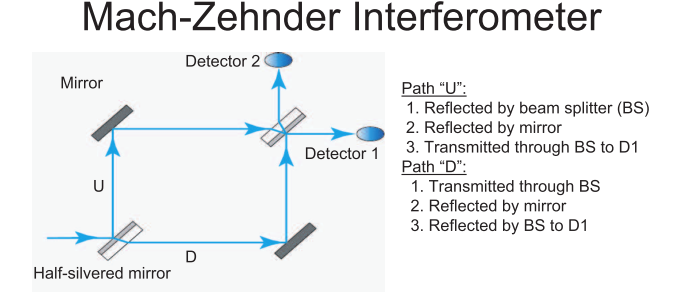
\includegraphics[scale=0.65]{Figures/mach-zender.png}
\caption{The Mach-Zehnder interferometer. \cite{dimaThesis}}
\label{mach-zehnder}
\end{figure}

As reflection results in a phase shift of $\pi$ and assuming transmission through the half-mirrors results in a phase shift of $\delta$ we easily calculate the phase differences of the two paths at the two detectors. At detector 1 and path $U$ there is a total of two reflections and a single transmission which results in a phase shift of $2\pi+\delta$. Similarly for path $D$ the phase shift is also $2\pi + \delta$. therefore at detector 1 there is constructive interference. At detector 2 path $U$ has a phase of $2\pi + 2\delta$ and path $D$ has a phase of $\pi + 2\delta$. Therefore at detector 2 there is destructive interference.\cite{dimaThesis}

\subsection{Three Blade Perfect Crystal Neutron Interferometer}
When inside the neutron interferometer it is useful to analyse the wavefunction as the sum of the two possible neutron paths which will be referred to as path one $\Psi_0 = \Ket{I}$ and path two $\Ket{II}$. The wavefunction inside the interferometer can be represented by\cite{dimaThesis} 
\begin{equation*}
\Psi = C_1e^{i\phi_1}\Ket{I} + C_2e^{i\phi_2}\Ket{II}
\end{equation*}
Where $\phi_i$ are the phase of each component and $C_i$ are the amplitudes of each component. Representing the amplitude of a Bragg transmitted wave as $t$ and the reflected amplitude as $r$, where $|r|^2+|t|^2 = 1$. The wavefunctions can be traced through the interferometer. Consider an initial neutron with wavefunction $\Ket{I}$ is incident on the first blade of the neutron interferometer. The resultant wavefunction is 
$$ te^{i\phi_{1_1}}\Ket{I} + re^{i\phi_{2_1}}\Ket{II}$$
This wavefunction is than incident on the second blade interferometer. Discarding the transmitted waves as they exit the interferometer, the resultant wavefunction is 
$$rte^{i\phi_{1_2}}\Ket{I} + rre^{i\phi_{2_2}}\Ket{II}$$
At the third and final blade, the geometry of the wave splitting superimposes path one and two onto each-other the two resultant beams are incident on two detectors, the upper detector known as the $O$ detector upon which the $O$ beam is incident and the lower which is known as the $H$ detector upon which the $H$ beam is incident. The resultant wave functions are 
\begin{equation}
\Ket{\Psi_O} = (rrte^{i\phi_1}+trre^{i\phi_2}) \Ket{I} \,\,\,\,\,\, \Ket{\Psi_H} = (trte^{i\phi_1}+rrre^{i\phi_2})\Ket{II}
\label{eq:beams}
\end{equation}
This results in an intensity at the $O$ detector of\cite{dimaThesis}
\begin{equation}
I_O \propto P(O|\Delta\phi) = \Braket{\Psi_O | \Psi_O} = |r|^4|t|^2(1+cos(\phi_1-\phi_2) = A(1+cos(\Delta\phi))
\label{eq:obeamintensity}
\end{equation} 
Where $A=|r|^4|t|^2$ and $\Delta\phi = \phi_1-\phi_2$. The resultant intensity for the $H$ beam is therefore 
\begin{equation}
I_H \propto P(H|\Delta\phi) = \Braket{\Psi_H | \Psi_H} = (|t|^4|r|^2 + |r|^6)-|r|^4|t|^2(cos(\phi_1-\phi_2)) = B - Acos(\Delta\phi)
\label{eq:hbeamintensity}
\end{equation}
Where $B=|t|^4|r|^2 + |r|^6$. 

The contrast of the neutron interferometer detectors is defined as 
\begin{equation}
C = \frac{\text{max}(I)-\text{min}(I)}{\text{max}(I)+\text{min}(I)}
\label{eq:contrastdefinition}
\end{equation}
Clearly than the contrast of the $O$ beam will be $1$ in the ideal case. However, the contrast of the $H$ beam will depend on the size of the reflection coefficient $r$. 
\begin{equation}
C_O = 1 \,\,\,\,\,\, C_H = \frac{|r|^4|t|^2}{|t|^4|r|^2+|r|^6}
\label{eq:contrasts}
\end{equation}
In (\ref{eq:hbeamintensity},\ref{eq:obeamintensity}) the intensities account for the loss of neutrons due to the transmitted neutrons in the second blade which exit the interferometer. This is apparent as 
$I_O+I_H \neq 1$. If the assumption is made that information is not lost with the exit of those neutrons the intensities can be reformulated by treating the second blades as ideal mirrors resulting in the new intensity formulation of\cite{dimaThesis}
\begin{equation}
I_O \propto P(O|\Delta\phi) = 2|rt|^2(1+cos(\Delta\phi)) \,\,\,\,\, I_H \propto P(H|\Delta\phi) = (|r|^4+|t|^4)-2|rt|^2cos(\Delta\phi)
\label{eq:normalizedIntensities}
\end{equation}
This revised intensity equation satisfies the property that $P(O|\Delta\phi)+P(H|\Delta\phi) = 1$. 
\subsection{Phase Flag}
\label{sec:phaseflag}
Utilizing the phase shift due to the neutron beam passing through a perturbing potential it is possible to analyse materials via the induced phase shift. 

\begin{figure}[ht!]
\centering
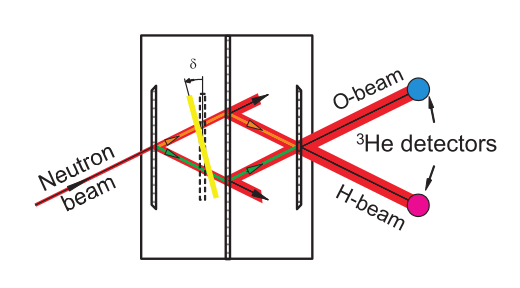
\includegraphics[scale=0.7]{Figures/phase_flag.png}
\caption{Neutron interferometer with a phase flag \cite{dimaThesis} }
\label{fig:phaseflag}
\end{figure}

As seen in fig(\ref{fig:phaseflag}) the two paths will pass through the phase flag. Providing the angle of the phase flag $\delta$ is not equal to zero the paths $D_1$ and $D_2$ will accrue a phase shift due to the different path lengths inside the material. The path lengths of the up and down beams are given by 
\begin{equation}
d_1 = \frac{D}{cos(\theta_B -\delta)} \,\,\,\,\, d_2 = \frac{D}{cos(\theta_B +\delta)}
\label{eq:phase_path_lengths}
\end{equation}
Where $D$ is the thickness of the phase flag, $\theta_B$ is the scattering Bragg angle of the two neutron beams relative to the horizontal, and $\delta$ is the angle of the phase flag relative to the vertical. Using these paths lengths and (\ref{eq:phase_shift_full}) the phase shift along each path are 
\begin{equation*}
\delta\phi_1 = \frac{Nb\lambda D}{ cos(\theta_B -\delta)} \,\,\,\,\, \delta\phi_2 = \frac{Nb\lambda D}{ cos(\theta_B +\delta)}
\end{equation*}
Which gives a relative phase between the two beams of 
$$\Delta\phi = Nb\lambda D \left(\frac{1}{cos(\theta_B -\delta)} - \frac{1}{cos(\theta_B +\delta)}\right) = $$
\begin{equation}
=-2NbD\lambda \frac{sin(\theta_B)sin(\delta)}{cos^2(\theta_B)-sin^2(\delta)} \approx (CONSTANT)\times \delta = C\delta
\label{eq:relative_phase}
\end{equation}
It should be noted that as (\ref{eq:relative_phase}) relies on a small angle approximation, the result only hold for approximately $\delta=0..\pi/10$. Due to this restriction of phase flag angles to have full control of the phase we require that
\begin{equation}
C\times  \geq \frac{2\pi}{\frac{\pi}{10}} = 20
\
\end{equation}
Using this result the intensity at the $O$ and $H$ detectors become 
\begin{equation}
I_O \propto  P(O|\Delta\phi,\delta) = A(1+cos(\Delta\phi)+C\delta) \,\,\,\,\, I_H \propto P(H|\Delta\phi,\delta) = B - Acos(\Delta\phi+C\delta)
\label{eq:intensities_phase_shift}
\end{equation}
The contrast of the neutron interferometer is a function of the phase flag angle and measured intensities at the neutron detectors\cite{noise_neutron}
\begin{equation}
C_0 = \frac{\text{max}[D_0(\delta)] - \text{min}[D_0(\delta)]}{\text{max}[D_0(\delta)] + \text{min}[D_0(\delta)]}
\label{eq:contrast}
\end{equation}
Where $D_0$ is the detected neutron intensity at the $O$ detector. Similarly to the case without a phase flag, the maximum contrast for the $O$ beam is $1$ and the H beam depends on the coefficient $r$. 
\subsection{Neutron Wave Guides}
\label{sec:waveguide}
As neutrons are a wave, similarly to light the obey Snell's Law 
\begin{equation}
n_1sin(\theta_1) = n_2sin(\theta_2)
\label{eq:snellslaw}
\end{equation}
Total reflection will occur when 
$$sin(\theta_2)= \frac{n_1}{n_2}sin(\theta_1)\le 0 \,\,\,\,\, \forall 0<\theta<\pi$$
As $max(sin(\theta_1))=1$ occur when $\theta_1=\frac{\pi}{2}$, using (\ref{eq:indexofrefraction}) the condition for total reflection in air where $n_1\approx1$ is  
\begin{equation}
V(x)> E_\perp
\label{eq:interalreflection}
\end{equation}
Therefore given a material with large enough values for $N$ and $b$ it is possible to design a waveguide for neutrons as they will simply reflect back and forth inside the guide. 

\begin{figure}[ht!]
\centering
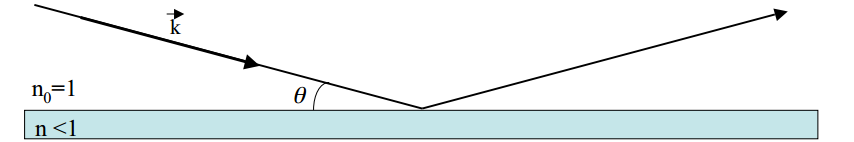
\includegraphics[width=\textwidth]{Figures/waveguide.png}
\caption{Neutron waveguide under the assumption that there is no Bragg scattering and the absorption is negligible \cite{waveguide} }
\label{fig:waveguide}
\end{figure} % Background Theory 

\chapter{Contrast Improvement of Neutron Interferometry Measurements} % Write in your own chapter title
\label{Chapter2}
\lhead{Chapter 2. \emph{Contrast Improvement of Neutron Interferometry Measurements}} % Write in your own chapter title to set the page header

\subsection{Probabilistic Models}
Ever since Max Born presented what would become to be known as the Born interpretation, quantum mechanics has become a science of probabilities. The Born rule states that the probability of measuring an eigenvalue $\lambda_i$  of an observable corresponding to a hermitian operator $A$  will be 
\begin{equation}
p(\lambda_i) = \Braket{\Psi|P_i|\Psi}
\label{eq:bornrule}
\end{equation}
This can be seen by applying the spectral theorem to $A$\cite{linear}
\begin{equation}
A = \lambda_1 P_1 + \lambda_2 P_2 \cdots \lambda_i P_i
\end{equation}
Where $P_i$ are the orthogonal projections of $A$ onto the eigenspace corresponding to $\lambda_i$. As $I = P_1 + P_2 \cdots + P_i$ and $\Braket{\Psi|\Psi} = 1$ given a probabilistic interpretation of the inner product. 
\begin{equation}
\Braket{\Psi|I|\Psi} =\Braket{\Psi|P_1|\Psi} + \Braket{\Psi|P_2|\Psi} + \cdots +\Braket{\Psi|P_i|\Psi}  = 1
\end{equation}
Given this result the interpretation may be made that 
\begin{equation*}
\Braket{\Psi|A|\Psi} = \lambda_1 \Braket{\Psi|P_1|\Psi} + \lambda_2\Braket{\Psi|P_2|\Psi} + \cdots +\lambda_i\Braket{\Psi|P_i|\Psi} =\lambda_1 p(\lambda_1) + \lambda_2p(\lambda_2) + \cdots +\lambda_ip(\lambda_i) = \bar{\lambda} 
\end{equation*}
Therefore it is quite easy to see where the Born rule arises. It is therefore clear that the Born interpretation opens physics up to the world of statisticians and their probabilities. Using techniques from statistics it is possible that improvements in neutron interferometer contrast may be made. 
\section{Baye's Theorem} 
Baye's theorem is a very interesting statistical method that is useful for predicting the accuracy of statistical models given event data. The generic form of Baye's Thereom is 
\begin{equation}
P(A|B) = \frac{P(B|A)P(A)}{P(B)} 
\label{eq:bayes}
\end{equation}
What this says is that given an event $B$ occurring from a set of events $\mathcal{E}$, the posterior probability that the model $A$ describing it is the most likely model in the set of models $\mathcal{M}$ is the probability of event $B$ occurring according to model $A$ multiplied by the prior likelihood of model $A$ and normalized by the total probability of event $B$ occurring according to all models in set $\mathcal{M}$.\cite{bayes}

This is an incredibly powerful theorem as it allows a set of models to be analysed statistically to determine the correct model with an actual likelihood of correctness given event data. A broad range of models can be tested and as more data rolls in the likelihood of the correct model to describe the system will rise.

There are discrete and continuous forms of Baye's theorem, however in this case only the discrete form is of interest. 
\begin{equation}
P(A_i|B) = \frac{P(B|A_i)P(A_i)}{\sum \limits_j P(B|A_j)P(A_j)}
\label{eq:discretebayes}
\end{equation}
\begin{figure}[ht!]
\centering
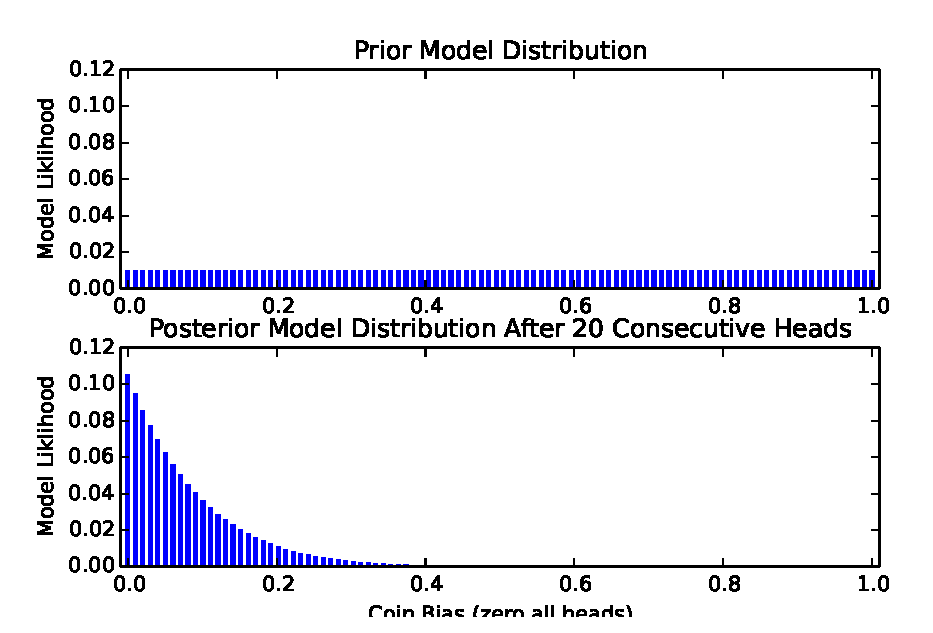
\includegraphics[scale=0.5]{Figures/bayes.eps}
\caption{Example prior and posterior distribution for a set of coin flip models that samples 10 heads flips in a row}
\label{fig:bayes}
\end{figure}
\section{Q-Infer}
\subsection{Interaction with NI-Engine}
\subsection{GPU Implementations of Likelihood functions} % Experimental Theory

% Chapter 4

\chapter{Experimental Setup} % Write in your own chapter title
\label{Chapter4}
\lhead{Chapter 4. \emph{Experimental Setup}} % Write in your own chapter title to set the page header


\section{The Neutron Interferometer}
The neutron interferometer that this thesis refers to is located at the Neutron Interferometry and Optics facility (NIOF) at the National Institute of Standards and Technology (NIST) in Gaithersburg, MD. 
\subsection{NIST}
\subsection{Reactor}
NIST operates a 20MW split-core research reactor. Neutrons of approximate energy $1 MeV$ are emitted during $^{235}U$ fission and then thermalized using heavy water ($D_2O$) as a moderator. This brings the neutrons to room temperature as discussed in (\ref{sec:thermal}). At the reactor core the peak thermal neutron flux is $4\times 10^{14} neutrons/cm^2$. The reactor is operated on a seven week cycle during which it is operated at full power for 38 days and then followed by 11 days of refuelling and maintenance operations. 

As the longer wavelength of cold neutrons ($\lambda>1.8\AA$ and $E<25meV$) is often desired for condensed matter study there is a cold moderator installed next to the core. The thermal neutrons scatter with liquid hydrogen at $20K$ and exit with a Maxwellian distribution of characteristic temperature of $34K$. 

There are eight thermal neutron ports available for lab use. The neutrons are transported to the instruments in the NCNR hall using neutron guides. The neutron interferometer facility is located on the NG7 guide shown in figure (\ref{fig:guides}). The guides are of a rectangular cross-section and are produced by gluing together meter long sections of $100nm$ thick $^{58}Ni$ optically-flat borated glass plates. $^{58}Ni$ is used due to its large neutron reflective potential. 
$$V = \frac{2\pi*\hbar^2}{m}\rho=\frac{2\pi\hbar^2}{m}\frac{1}{V}\sum\limits_{i} b = 335neV$$



\subsection{Motors and Actuators}
The neutron interferometry lab uses a variety of motors and actuators that allow experimental parameters to be controlled over the wire. Depending on the device communication is achieved via analog or digital protocols.
\subsubsection{Newport 301}

The Newport ESP301 is a three axis motion controller and driver.\cite{esp301manual} It can drive both DC servo motors and 2-phase stepper motors at up to 3 amps. It has a 1000x micro-step resolution per axis which allows very fine grained control of movements which is necessary for precision measurements. The Newport ESP 301 is primarily used to drive servo motors that orient the phase flag in the neutron interferometer. Precise angular control is a must as this is one of the primary experimental parameter. The device can also be used to control the interferometry stage to orient it. 

The Newport device utilizes encoder feedback built into servos to obtain precise positional feedback. While most Newport brand motors will automatically supply their configuration information, the equipment at NIST is not necessarily compatible in such a way. Therefore advanced configuration must be supplied by the device programmer. 

The ESP301 is controllable via a fairly extensive language of approximately 100 commands, a large portion of which are necessary for the device to be controlled successfully. Valid configuration information must be supplied. Commands are transmitted via ASCII characters according to the selected protocol. Supported protocols are serial RS232C, USB and IEEE488 with delays of $7-30ms$,$3.5ms$ and $1ms$ respectively.

\begin{figure}[ht!]
\centering
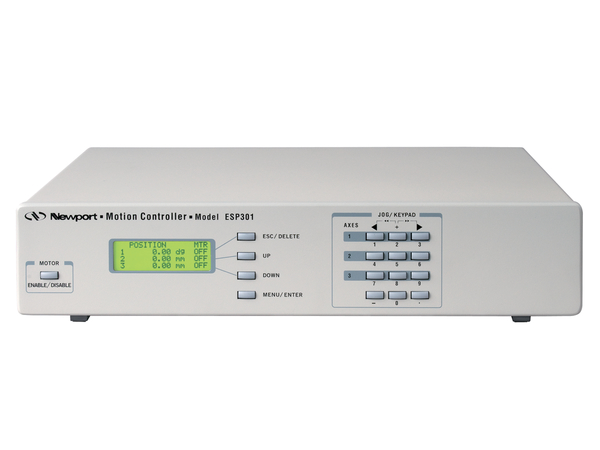
\includegraphics[scale=0.5]{Figures/esp301.jpg}
\caption{Newport ESP301 three axis motion controller}
\label{fig:esp301}
\end{figure}
\subsubsection{Kepco Power Supply}
Kepco series ATE power supplies are used to control a variety of devices in the interferometry lab. Specifically the 15-6M and 36-15M models are used and are rack mounted. The models are rated at ($0$-$15V$,$0$-$6A$,$50W$) and ($0$-$36V$,$0$-$15A$,$500W$) respectively.\cite{kepco} The models are controllable via an analog input line that sets the supply output as a linear function of the input from $0$-$10V$. Additionally there is a crowbar voltage controller which allows a maximum voltage to be set in a similar manner. The Kepco supplies are controllable via DACs which are managed via a LabJack. 
\subsubsection{LabJack}
The LabJack is a low cost measurement and automation platform. Specifically NIST will use the U3-LV variant. The U3-LV provides up to 16 analog inputs, 2 analog outputs and up to 20 digital I/O pins. The analog inputs accept voltages from $0$-$3.6V$ and the onboard DACs outputs from $0$-$5V$. The LabJack devices are easily controlled via a Python API. 

In Addition to the LabJack the LJTick-DACs, a DAC made to be digitally controlled by LabJack devices are used to provide control inputs to devices such as the Kepco power supplies. The LJTick-DAC outputs $\pm10V$  controllable by the LabJack pins in which it is inserted too. Each LJTick-DAC provides two DACs. 
\begin{figure}[ht!]
\centering
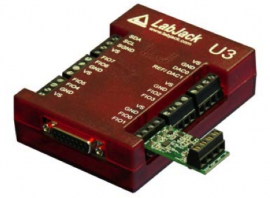
\includegraphics[scale=0.5]{Figures/labjack.png}
\caption{Labjack U3 with LJTick-DAC}
\label{fig:labjack}
\end{figure}
\subsection{Sensors}
As the likelihood method for the contrast measurement is a function of the temperature and humidity of the interferometer chamber, a variety of measurements must be taken using many different sensors.
\subsubsection{EI1050 Temperature and Humidity Probe}
The EI1050 is a digital temperature and humidity probe produced by LabJack. While its protocol is open source, it has been designed to be used with a LabJack device and sample code has been provided. The device is not especially accurate as it is rated at $\pm0.5^{\circ}$ and $\pm3.5\%$ humidity at ranges from $-40$-$120C$ and $0$-$100\%$ humidity. It is still useful to provide a quick and easy measurement. 
\subsubsection{Stanford Research Systems CTC100 Temperature Controller}
The SRS CTC100 is a cryogenic temperature controller. It provides four sensor inputs, four analog outputs and six feedback control loops. Temperature readings are made by thermistor sensors and heating is provided by resistive heaters. The device is programmable using USB, Ethernet and either GPIB or RS-232 inputs. Commands are provided via ASCII commands.  
The thermistor temperature readings are very accurate with an accuracy of $\pm0.25\Omega$ for a $300\Omega$ thermistor. The CTC100 automatically supplies the mean and standard deviation of sampled temperatures. 
\begin{figure}[ht!]
\centering
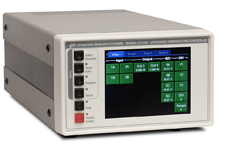
\includegraphics[scale=1.0]{Figures/ctc100.jpg}
\caption{Stanford Research Systems CTC100: Cryogenic Temperature Controller}
\label{fig:ctc100}
\end{figure}
\section{NI-Engine}
The current system at the NIST interferometry lab uses an Excel spreadsheet connected via ActiveX to closed source controller code. This system only controls the bare minimum of experimental hardware and is very inflexible. The system is not easily extensible and the software design principles are very poor. As the contrast improvement experiment requires many different sensor inputs and system controllability for many different measurement cases, it would have been a tremendous task to implement into the current system. 

Ni-Engine attempts to solve the problems of the previous system for the proposed experiment and future lab researchers. NI-Engine is an experimental neutron interferometry control system programmed in Python using open source libraries and software design principles.
\subsection{Design Requirements}
\label{sec:requirements}
The core design requirement of NI-Engine are to be a complete, easy to use neutron interferometry experimental control system. In order fulfil this core requirement the software had to fulfil these requirements: 
\begin{itemize}
  \item Be able to communicate with and control a large range of hardware in a manner that allows powerful functionality while hiding the inherent complexity. 
  \item Handle experimental setup and configuration via configuration files such that an experimental setup is easily repeatable given an identical configuration. 
  \item Handle the collection and storage of experimental data. Experimental data will be large, possible into the $10+GB$ range. Should allow for multiple identical experiments to be performed sequentially.
  \item Execution of software functionality must be fast and allow for experiment running times to be dominated by hardware measurement and control, rather than software running time. 
  \item Software must be able to run for long periods of time with consistent memory requirements.
  \item Data should be collected and stored with units available to avoid confusion.  
  \item Should be modular. Outside researchers should be able to modify software to their own requirements. ie. addition of new hardware, file formats, data types. 
  \item Software must have extensive documentation and example code. Researchers should be able to utilize without extensive outside help.  
\end{itemize}
These design requirements had to be taken into account when designing and programming Ni-Engine
\subsection{Language and Software Library Choices}
\subsubsection{Language}
Given the design requirements outlined in (\ref{sec:requirements}) it is clear that the system required is quite extensive. Python\cite{python} was selected as the development language for Ni-Engine. Python was selected for a variety of reasons including 
\begin{itemize}
\item Python is very easy to learn and use. Its syntax style allows newcomers the ability to quickly write code, while still allowing experts powerful expressibility. 
\item Python's code is extremely legible and the nature of its syntax naturally generates readable code. 
\item Python has many powerful libraries available that when used allow rapid development of complex software without the complexity of rolling ones own solution. 
\item Python has a large and help community. 
\item It is very easy to interface with C based code if performance is desired. 
\item Python is object oriented which when used correctly allows simple creation of modular and extensible software. 
\item Python is dynamically typed and evaluated which allows rapid iteration and ease of use at the cost of performance and security. 
\end{itemize}
While the use of python does come at some costs, namely memory and CPU performance, on a whole the choice of language provided enormous benefits.

\subsubsection{Software Libraries}
Due to the nature of an experimental system composed of heterogeneous hardware there is a lot of complexity in communicating with hardware over different communication channels. To overcome this challenge the library  InstrumentKit\cite{instrumentKit} was used. InstrumentKit allows identical commands to be sent over a variety of different communication channels at a high level of abstraction. It was a much more simple matter to contribute communication code for necessary sensors and hardware to InstrumentKit and then just utilize the library. As Ni-Engine must handle large volumes of data and manipulate this data, Numpy\cite{numpy} was used for its efficent handling of arrays in Python and the variety of methods it provides. To store this data the first file format to be implemented was HDF5\cite{hdf5}, which is a version of the Hierarchical Data Format. HDF5 was designed for the storage of large amounts of numerical data. Additionally, it provides an easily navigable hierarchical file system. Creation and manipulation of HDF5 files was facilitated by the memory efficient H5py\cite{h5py} library for Python. As the main goal of the system is to handle experimental data that is often associated with physical units of measurement Python units\cite{units} was used. Units allows the wrapping of Python data types and Numpy arrays in physical units, and performs the necessary unit operations when performing operations between data types of units. 

As extensive documentation is a core design requirement of Ni-Engine, it was essential that a documentation generation library be used throughout development. Sphinx\cite{sphinx}, the De facto Python standard for documentation pulls in-code comments and generates relational documentation in a variety of formats including html and pdf formats. 
\subsection{System Architecture}
\subsection{Documentation}
\section{Q-Infer}
\subsection{Interaction with NI-Engine}
\subsection{GPU Implementations of Likelihood functions}

 % Experimental Setup

% Chapter 5

\chapter{Discussion and Conclusion} % Write in your own chapter title
\label{Chapter5}
\lhead{Chapter 5. \emph{Discussion and Conclusion}} % Write in your own chapter title to set the page header

\section{Results}
While it was not possible to carry out our proposed experiment to test the algorithm described in section (\ref{sec:robusthamiltonian}) it was still possible to model and simulate the behaviour of the algorithm for the proposed system. Our model model attempted to take into account imperfections in the experimental setup such as variable offsets, temperatures, humidities, and phase constants. The derived model for probability of detection at the O-detector is given by (\ref{eq:finalmodel}).

Simulation of the behaviour of the MCMC algorithm was performed on a variety of chosen parameter sets for the model in order to verify if in theory the algorithm would be able to adequately converge on a valid approximate solution. Simulations demonstrated that the algorithm would be able to greatly decrease the Bayes risk and converge on the true parameter set in all tested cases.   

The most interesting aspect of the algorithm and our results is that of experimental design. The Robust Online Hamiltonian Learning algorithm allows future experimental parameters to be chosen to maximize the amount of information gain and thus reduce the Bayes risk to a much greater degree with each additional experiment. This is especially useful when experiments require a long time to perform for different experimental parameters and the time of simulation is much less than that of performing additional experiments. As could be seen in fig(\ref{fig:adaptivetimes}) the algorithm could rapidly converge on the true parameter set in as little as $50$ experiments, rivalling the accuracy of the naive test of $2^15$ phase flag settings experiment. Analysis of the probability density functions, shows that the majority of probability density is concentrated around the true values of parameters. 

A downside of the experimental adaptive design is the simulation time required greatly increases. The selection of experimental parameters to maximize information gain greatly increases the computational time. Therefore adaptive experimental design will only actually increase the average information gain per time unit if the cost of simulation is less than the time taken to perform enough experiments to equal the information gained through measurement of choice experimental parameters. In section (\ref{sec:gpu}) we explored implementing the likelihood functions on graphics processing units for GPGPU calculations. Although the speed-up experienced was lower than expected, there are almost certainly large optimizations to be made as our approach was relatively naive and experimental. Additional ways in which the likelihood evaluation speed could be increased is through field programmable gate arrays or application specific circuits (ASIC). 

\section{Ni-Engine}
Ni-Engine was programmed to be compatible with Q-Infer in order to perform the experimental verification of our simulations. Unfortunately due to scheduling conflicts and the priorities of the research group, both Q-Infer and Ni-Engine have to yet to be put to use at NIST. However, it is anticipated that at some point in the near future, the software and hardware will be installed and we will be able to perform our experimental verification. 

Ni-Engine was extensively tested at IQC with the real hardware. While, experiments were not able to be performed at the neutron interferometry lab, simulated experiments were performed with backups of the lab equipment. This allowed real experiments to be scripted, data measured and stored. This, along with the thorough documentation provided, allows me to believe that Ni-Engine will have widespread use in the lab when installed due to the benefits it provides over the current experimental system. 

\section{Application to Quantum Information and Fundamentals}
The algorithm implemented by Q-Infer has the potential to be very useful in the field of experimental quantum mechanics. Most quantum experimental setups in existence have been modelled mathematically, however all models require that the parameters of the particulars of the system be discovered. This is normally a very experimentally and computationally challenging task as many experiments must be done to gain sufficient information to fit the parameters to the system and fitting itself is a computationally intensive task. Our algorithm solves this issue and, even though it is using approximate probabilistic methods, allows the error in approximated parameters to be calculated. The amount of experiments required with this algorithm are often much less than would be required to characterise the system with quantum tomography. Provided the system has a model the proposed algorithm appears to be an excellent solution to the problem of discovering system parameters. 


 % Results and Discussion and Conclusion





%% ----------------------------------------------------------------
% Now begin the Appendices, including them as separate files

\addtocontents{toc}{\vspace{2em}} % Add a gap in the Contents, for aesthetics

\appendix % Cue to tell LaTeX that the following 'chapters' are Appendices

%% Appendix A

\chapter{Test System Specifications}
\label{app:testsystem}
\lhead{Appendix A. \emph{Appendix Title Here}}

The specifications of the test system are found in table (\ref{tab:testsystem}). 

\begin{table}[h!]
\begin{center}
\begin{tabular}{l*{6}{c}r}
Component Type            & Model  \\
\hline
\\
CPU & Intel i5 2500k overclocked \@ 3.9GHz \\
GPU & Nvidia GTX 560ti \\ 
Hard Drive & OCZ Twin Vertex II SSD \\
RAM & 12GB 1600Mhz \\
Motherboard & MSI P67A-GD65 \\
\end{tabular}

\caption{Test system specifications}
\label{tab:testsystem}
\end{center}
\end{table}	% Appendix Title

%\input{./Appendices/AppendixB} % Appendix Title

%\input{./Appendices/AppendixC} % Appendix Title

\addtocontents{toc}{\vspace{2em}}  % Add a gap in the Contents, for aesthetics
\backmatter

%% ----------------------------------------------------------------
\label{Bibliography}
\lhead{\emph{Bibliography}}  % Change the left side page header to "Bibliography"
\bibliographystyle{unsrtnat}  % Use the "unsrtnat" BibTeX style for formatting the Bibliography
\bibliography{Bibliography}  % The references (bibliography) information are stored in the file named "Bibliography.bib"

\end{document}  % The End
%% ----------------------------------------------------------------